\documentclass{beamer}

\usepackage[T1]{fontenc}
\usepackage[utf8]{inputenc}
\usepackage[english]{babel}
\usepackage{lmodern}

% Use Unipd as theme, with options:
% - pageofpages: define the separation symbol of the footer page of pages (e.g.: of, di, /, default: of)
% - logo: position another logo near the Unipd logo in the title page (e.g. department logo), passing the second logo path as option 
% Use the environment lastframe to add the endframe text
\usetheme[pageofpages=of]{Unipd}

\title{ \textbf{ \textit{SMKIT} } }
\subtitle{ \textbf{ \textit{Design and development of a social media kit} } }
\author[ \textbf{ \textit{Abdelilah Lahmer} } ]{ \textbf{ \textit{Lahmer Abdelilah} } }

\date{ \textbf{ \textit{December 12, 2024} } }

% The next block of commands puts the table of contents at the beginning of each section and highlights the current section
\AtBeginSection[]
{
  \begin{frame}
    \frametitle{Table of Contents}
    \tableofcontents[currentsection]
  \end{frame}
}



\begin{document}

% Make the title page
\frame{\titlepage}

% Insert the general toc
\begin{frame}{Table of Contents}
    \tableofcontents    
\end{frame}


\section{Introduction}
    \begin{frame}{Introduction to SMKIT}
        \vspace{0.5cm}
        \begin{itemize}
            \item \textbf{SMKIT} stands for \textbf{Social Media KIT}.
            \item A modular tool for automating social media and web content posting.
            \item Designed to process web and local pages, extract metadata, and generate posts for various social platforms.
        \end{itemize}

        \begin{center}
            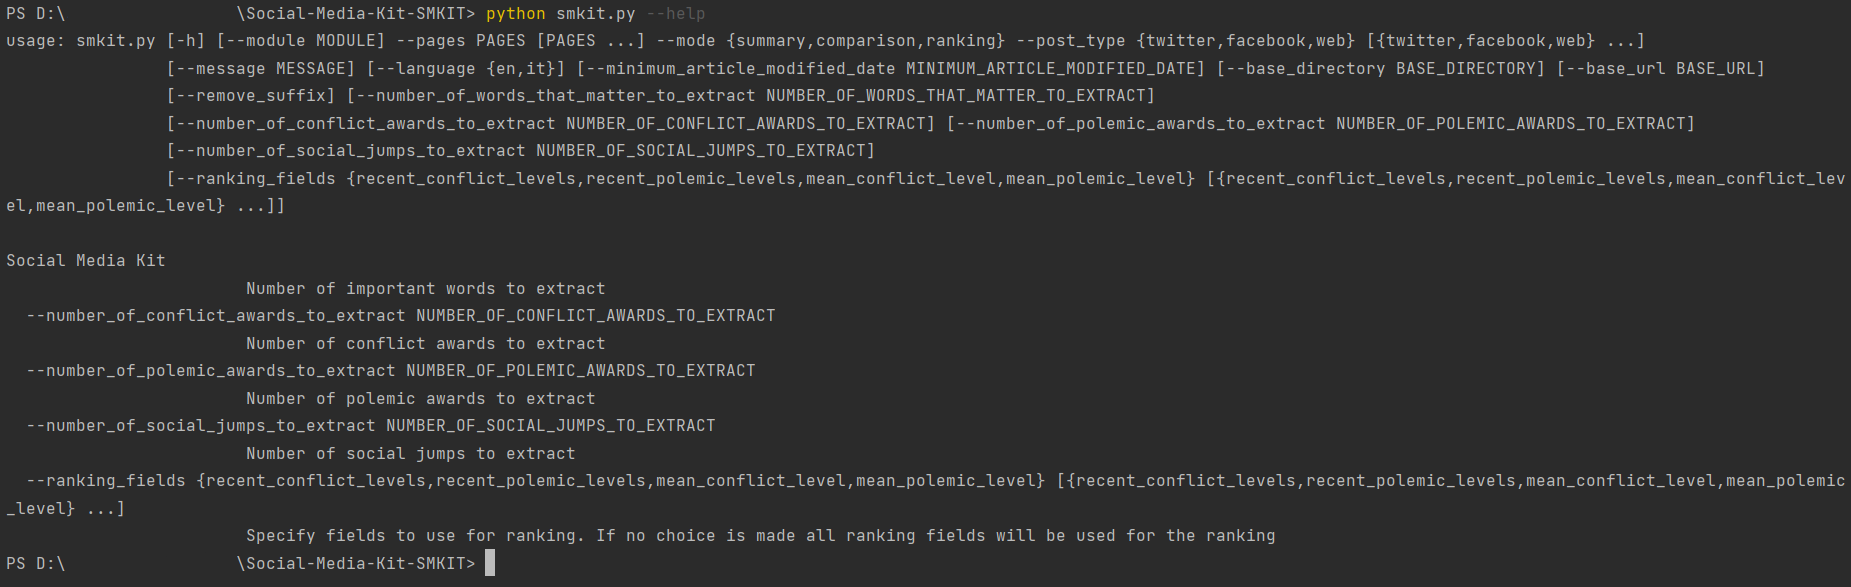
\includegraphics[width=\textwidth, keepaspectratio]{images/introduction_introduction_to_smkit_slide_image.png}
        \end{center}
    \end{frame}

    \begin{frame}{Background}
        \begin{columns}[T]
            \column{0.25\textwidth}
            \vspace{-0.25cm}
            \begin{center}
                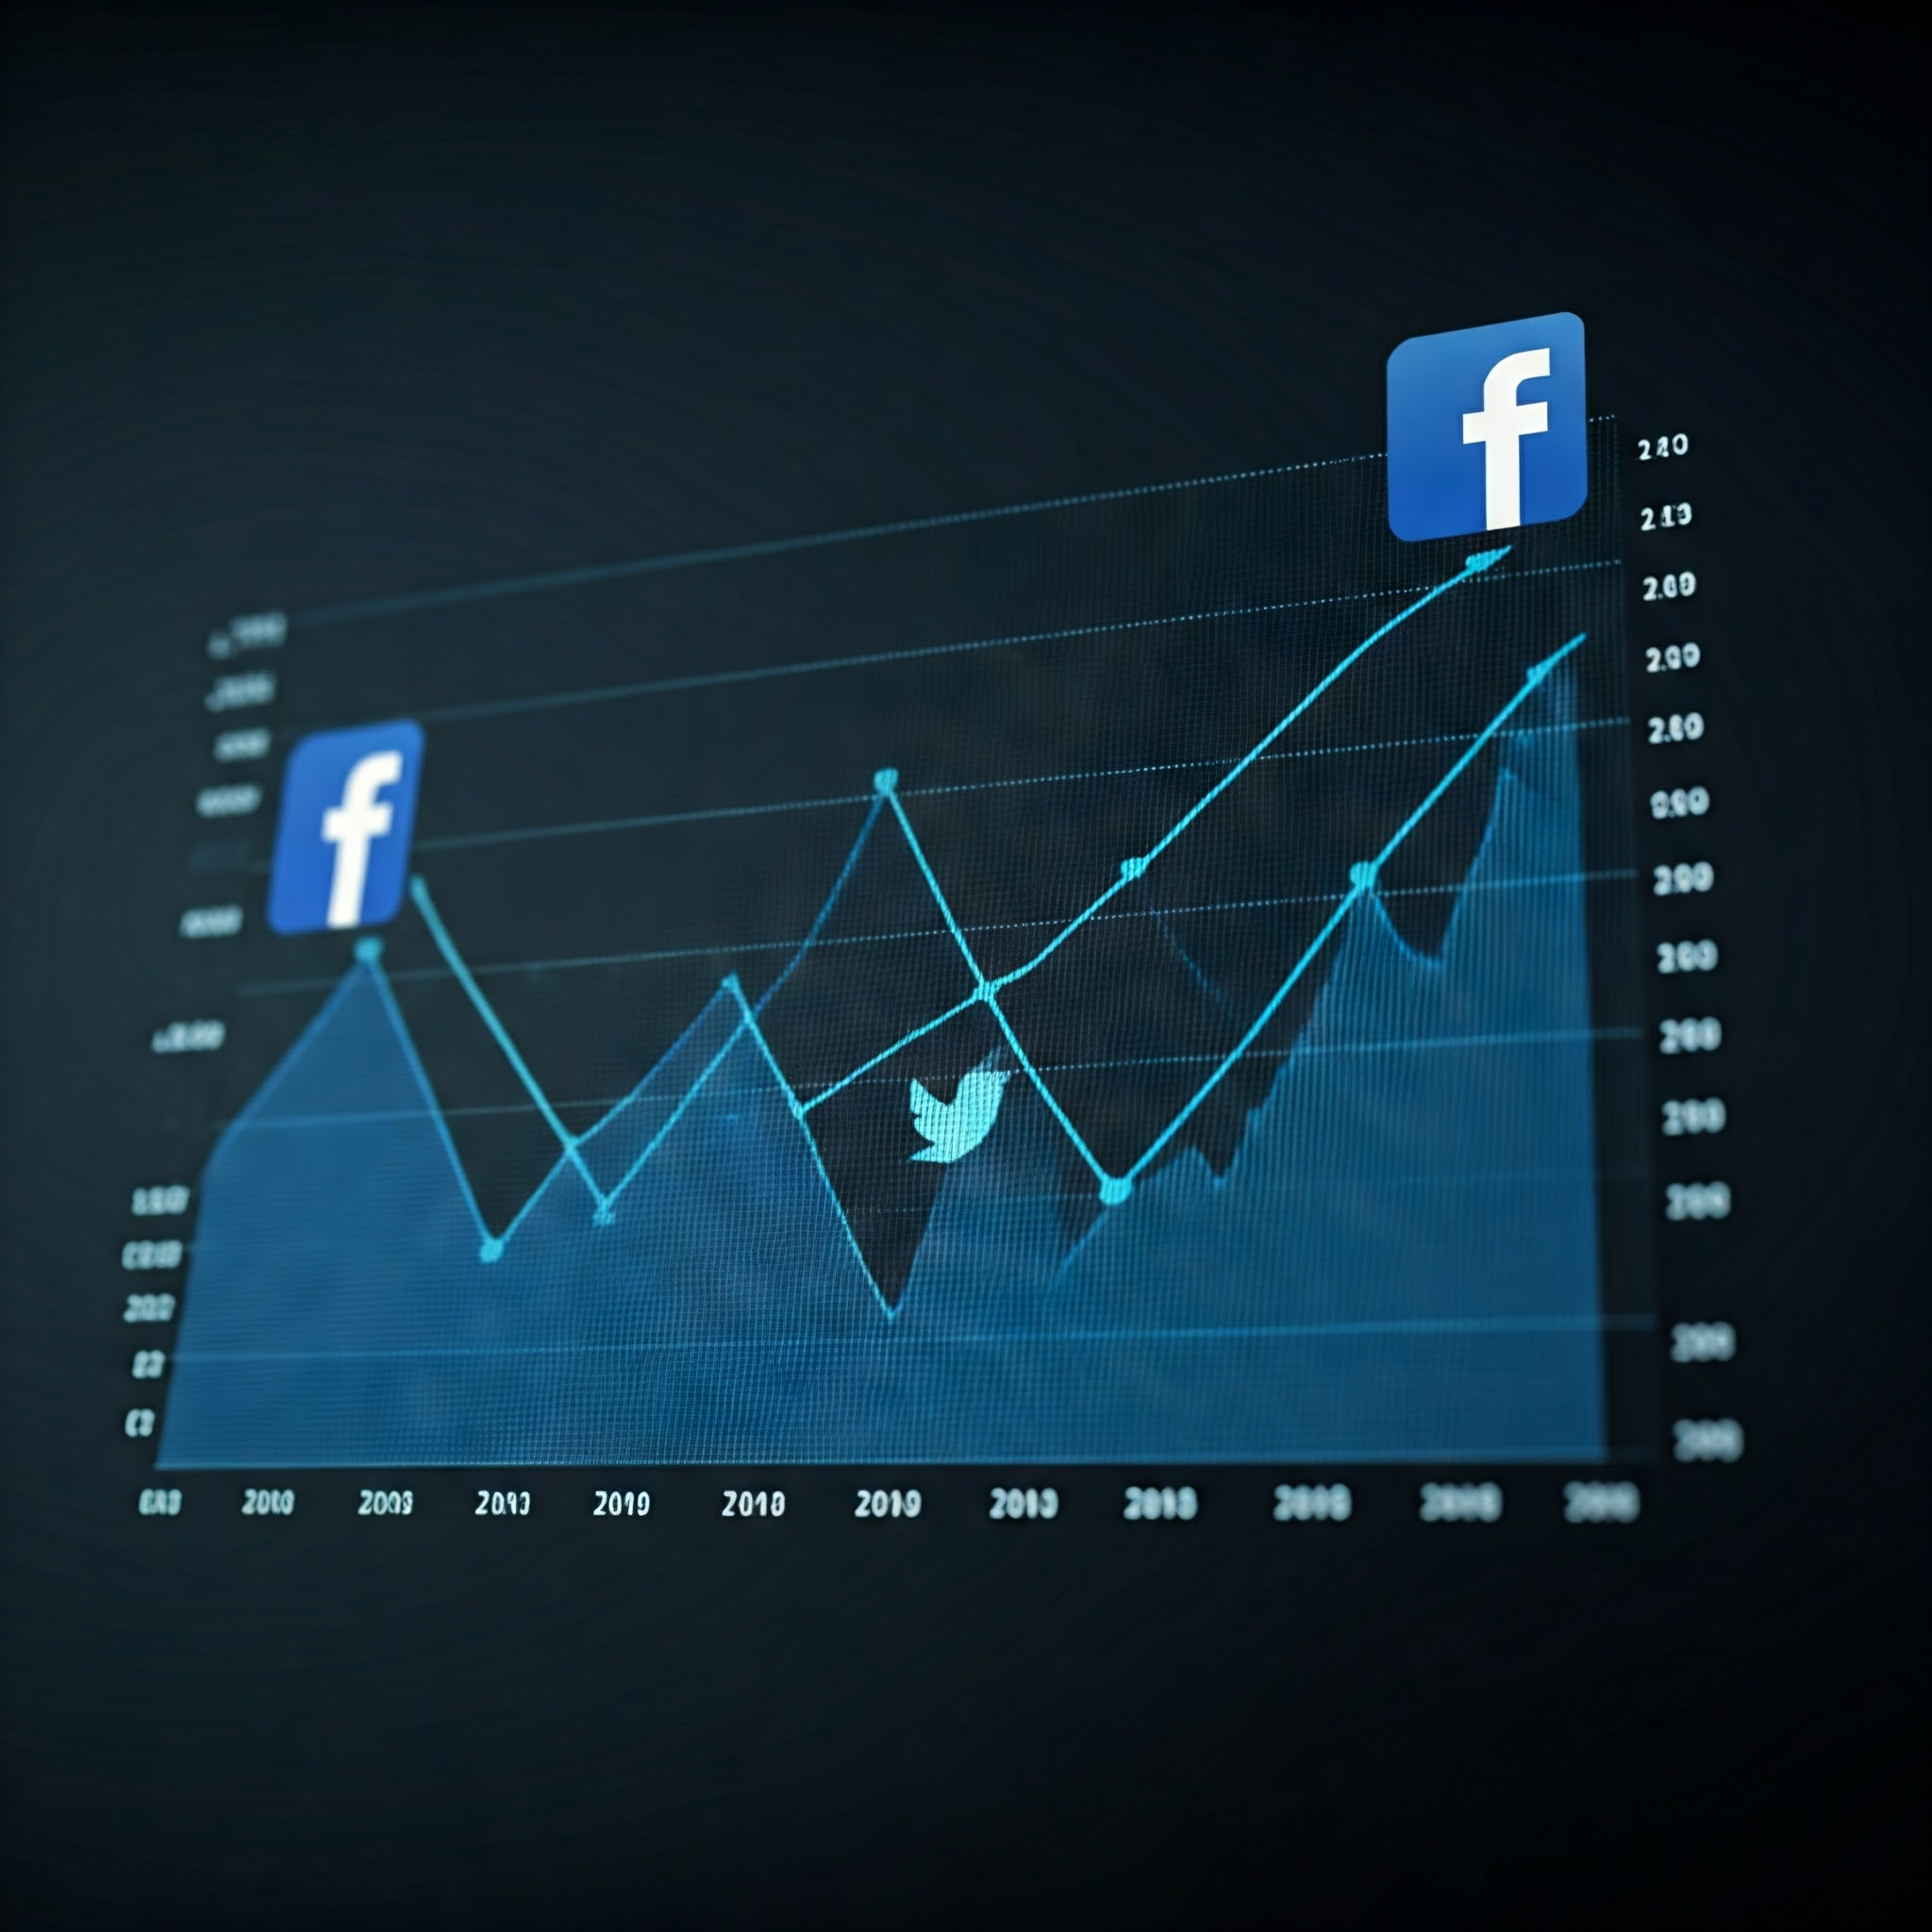
\includegraphics[width=1.35\textwidth, keepaspectratio]{images/introduction_background_slide_image.jpeg}
            \end{center}

            \column{0.75\textwidth}
            \vspace{0.5cm}
            \begin{itemize}
                \item \textbf{Rapid growth of web content and social media:}
                \begin{itemize}
                    \item Over 5.22 billion active social media users globally in 2024\**.
                    \item Platforms include Facebook, Twitter, LinkedIn, Instagram, and others.
                \end{itemize}
            \end{itemize}
        \end{columns}

        \vspace{0.5cm}
        \begin{itemize}
            \item \textbf{Challenges in content management and distribution:}
            \begin{itemize}
                \item Managing the volume of web content is impractical manually.
                \item Ensuring consistency across platforms requires efficient tools.
            \end{itemize}
        \end{itemize}

        \vspace{1.25cm}
        {\tiny \** Source: \url{https://datareportal.com/social-media-users}}
    \end{frame}

    \begin{frame}{Motivation}
        \begin{columns}[T]
            \column{0.27\textwidth}
            \hspace{-0.5cm}
            \vspace{0.2cm}
            \begin{center}
                
\includegraphics[width=1.63\textwidth, keepaspectratio]{images/introduction_motivation_slide_image.png}
            \end{center}

            \column{0.73\textwidth}
            \vspace{0.5cm}
            \begin{itemize}
                \item \textbf{Need for automation:}
                \begin{itemize}
                    \item Optimizes processes, reduces manual effort.
                    \item Ensures consistency and scalability through different platforms.
                \end{itemize}
            \end{itemize}
        \end{columns}

        \vspace{0.5cm}
        \begin{itemize}
            \item \textbf{Gaps in current tools:}
            \begin{itemize}
                \item Many tools focus on single platforms or lack in modularity.
                \item Inadequate metadata handling, particularly for non-standard websites.
                \item Poor adaptability to new platforms or content types.
            \end{itemize}
        \end{itemize}
    \end{frame}


\section{Preliminaries}
    \begin{frame}{What's Open Graph Protocol?}
        \begin{block}{What is Open Graph Protocol?}
        \begin{itemize}
            \item A protocol designed to make web pages more social-media friendly.
            \item Developed by Facebook to provide metadata for rich media previews.
        \end{itemize}
        \end{block}

        \begin{exampleblock}{Open Graph Examples}
            \begin{itemize}
                \item \textbf{og:title:} The title of the page.
                \item \textbf{og:description:} A short description of the page.
                \item \textbf{og:image:} The main image to represent the page.
                \item \textbf{og:url:} The canonical URL of the page.
            \end{itemize}
        \end{exampleblock}
    \end{frame}

    \begin{frame}{What is Negapedia?}
        \begin{block}{Overview}
            \begin{itemize}
                \item Negapedia is a unique platform that tracks and visualizes conflicts and controversies on Wikipedia.
                \item It provides insights into both historical and recent conflict/polemic trends across various topics.
            \end{itemize}
        \end{block}

        \begin{exampleblock}{Key Features of Negapedia}
            \begin{itemize}
                \item \textbf{Conflict Levels:} Measures the size of disputes and negative interactions within a Wikipedia page.
                \item \textbf{Polemic Levels:} Evaluates the emotional tone and hostility within community discussions about a topic.
                \item \textbf{Awards and Rankings:} Highlights the most polemic or debated topics.
            \end{itemize}
        \end{exampleblock}
    \end{frame}


\section{Problem Statement}
    \begin{frame}{Problem Statement}
        \begin{block}{Challenge}
            Managing the continuously growing web content and social media manually is time-consuming, inconsistent, and inefficient.
        \end{block}

        \vspace{0.5cm}

        \begin{alertblock}{Problem}
            Existing tools lack multi-platform integration, modularity, and effective handling of non-standard metadata formats.
        \end{alertblock}

        \vspace{0.5cm}

        \begin{exampleblock}{Solution}
            A scalable, modular solution like SMKIT can ensure consistency and adaptability across diverse content and platforms.
        \end{exampleblock}
    \end{frame}


\section{Objectives}
    \begin{frame}{Objectives}
        \begin{block}{Primary Objective}
            Develop SMKIT to automate and optimize social media and web content management.
        \end{block}

        \begin{itemize}
            \item \textbf{Automating Content Posting:}
                Reduce manual effort and ensure consistent scheduling.
            \vspace{0.3cm}
            \item \textbf{Multi-Platform Support:}
                Smooth integration with platforms like Twitter and Facebook.
            \vspace{0.3cm}
            \item \textbf{Metadata Extraction:}
                \begin{itemize}
                    \item Extract essential metadata like Open Graph tags.
                    \item Handle non-standard metadata efficiently.
                \end{itemize}
            \vspace{0.3cm}
            \item \textbf{Modularity and Scalability:}
                Support feature extensibility and increasing workloads.
        \end{itemize}
    \end{frame}


\section{Overview of SMKIT}
    \begin{frame}{Workflow}
        \begin{itemize}
            \item \textbf{Workflow Overview:}
                SMKIT operates in a modular structure with two main ones:
                \begin{itemize}
                    \item \textbf{Generic Module:} Handles Open Graph metadata extraction for diverse web pages.
                    \item \textbf{Negapedia Module:} Processes specific data tailored to the \href{http://www.negapedia.org/}{negapedia.org} platform.
                \end{itemize}
            \item Both modules feed into posting connectors for publishing on channels like Facebook, Twitter, or for creating websites.
        \end{itemize}

        \begin{center}
            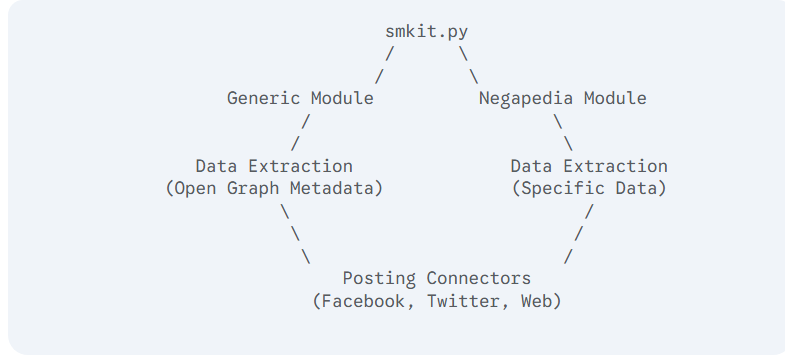
\includegraphics[width=0.85\textwidth, keepaspectratio]{images/overview_on_smkit_workflow_slide_image.png}
        \end{center}
    \end{frame}

    \begin{frame}{Features}
        \begin{itemize}
            \item \textbf{Metadata Extraction:}
                \begin{itemize}
                    \item Supports Open Graph tags (e.g., og:title, og:description, og:image).
                    \item Handles specific data structures for Negapedia platform.
                \end{itemize}
            \vspace{0.3cm}
            \item \textbf{Multi-Channel Posting:}
                \begin{itemize}
                    \item Supports posting to Facebook, Twitter, and Web channels.
                    \item Ensures channel-specific formatting and requirements.
                \end{itemize}
            \vspace{0.3cm}
            \item \textbf{Customizable Templates:}
                \begin{itemize}
                    \item Provides flexible templates for consistent branding across posts.
                \end{itemize}
            \vspace{0.3cm}
            \item \textbf{Modular Design:}
                \begin{itemize}
                    \item Allows seamless integration of new modules for additional functionality.
                    \item Scalable to accommodate new platforms and content types.
                \end{itemize}
        \end{itemize}
    \end{frame}


\section{Technical Implementation}
    \begin{frame}{Core Modules}
        \begin{block}{Generic Module}
            Extracts and processes Open Graph metadata from web pages. This module:
            \begin{itemize}
                \item Handles standard metadata tags (e.g., og:title, og:description, og:image).
                \item Implements fallback mechanisms for missing or non-standard metadata.
            \end{itemize}
        \end{block}

        \begin{block}{Negapedia Module}
            Specialized for the Negapedia platform.
            This module:
            \begin{itemize}
                \item Extracts structured data such as historical conflict and polemic metrics, awards, and rankings.
                \item Processes content using Negapedia-specific rules and formats.
            \end{itemize}
        \end{block}
    \end{frame}

    \begin{frame}{Posting Process}
        \begin{block}{Integration with APIs}
            SMKIT integrates seamlessly with social platform APIs for automated posting:
            \begin{itemize}
                \item \textbf{Facebook API}: Posts content with metadata, images, and descriptions using \textbf{facebook-sdk} for Python.
                \item \textbf{Twitter API}: Publishes concise posts with links, images, and hashtags using \textbf{tweepy} library  for Python.
            \end{itemize}
        \end{block}
    
        \begin{block}{Template Usage}
            Consistent branding and identity are achieved through customizable templates:
            \begin{itemize}
                \item Uniformity across platforms is achieved thanks to templates.
                \item Supports platform-specific adaptations and restrictions.
            \end{itemize}
        \end{block}
    \end{frame}


\section{Negapedia Module}
    \begin{frame}{Modes of Operation}
        \textbf{Modes of Operation}
        
        The Negapedia Module can be called using three modes:
            \begin{itemize}
                \item \textbf{summary:}
                    Extracts key insights from individual Negapedia pages, such as:
                    \begin{itemize}
                        \item Historical conflict levels.
                        \item Recent polemic levels.
                        \item Top awards and rankings.
                    \end{itemize}
                \item \textbf{comparison:}
                    Compares data across two Negapedia pages, showcasing differences in:
                    \begin{itemize}
                        \item Conflict or polemic metrics.
                        \item Social jumps or awards.
                    \end{itemize}
                \item \textbf{ranking:}
                    Ranks multiple Negapedia pages based on selected metrics:
                    \begin{itemize}
                        \item Generates sorted lists on quantitative insights, such as recent conflict levels or mean polemic levels.
                    \end{itemize}
            \end{itemize}
    \end{frame}


\section{SMKIT in Action}
    \begin{frame}{Twitter Post}
        Post generated using \textbf{Generic Module} in \textbf{Summary Mode}.
        \begin{center}
            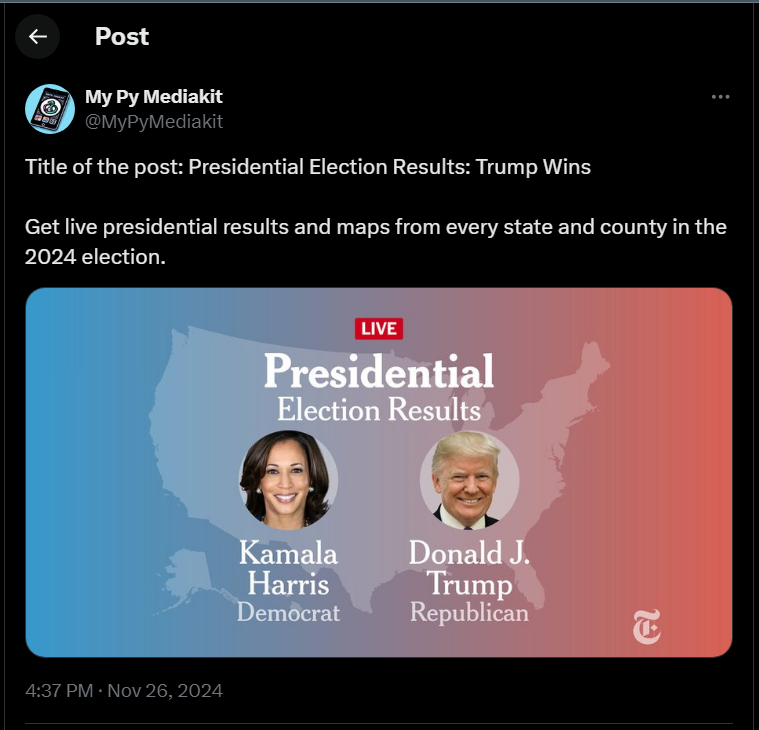
\includegraphics[width=0.67\textwidth, keepaspectratio]{images/twitter_generic_summary_post_screenshot.png}
        \end{center}
    \end{frame}

    \begin{frame}{Web Page Post}
        Page generated using \textbf{Negapedia Module} in \textbf{Comparison Mode}.
        \begin{center}
            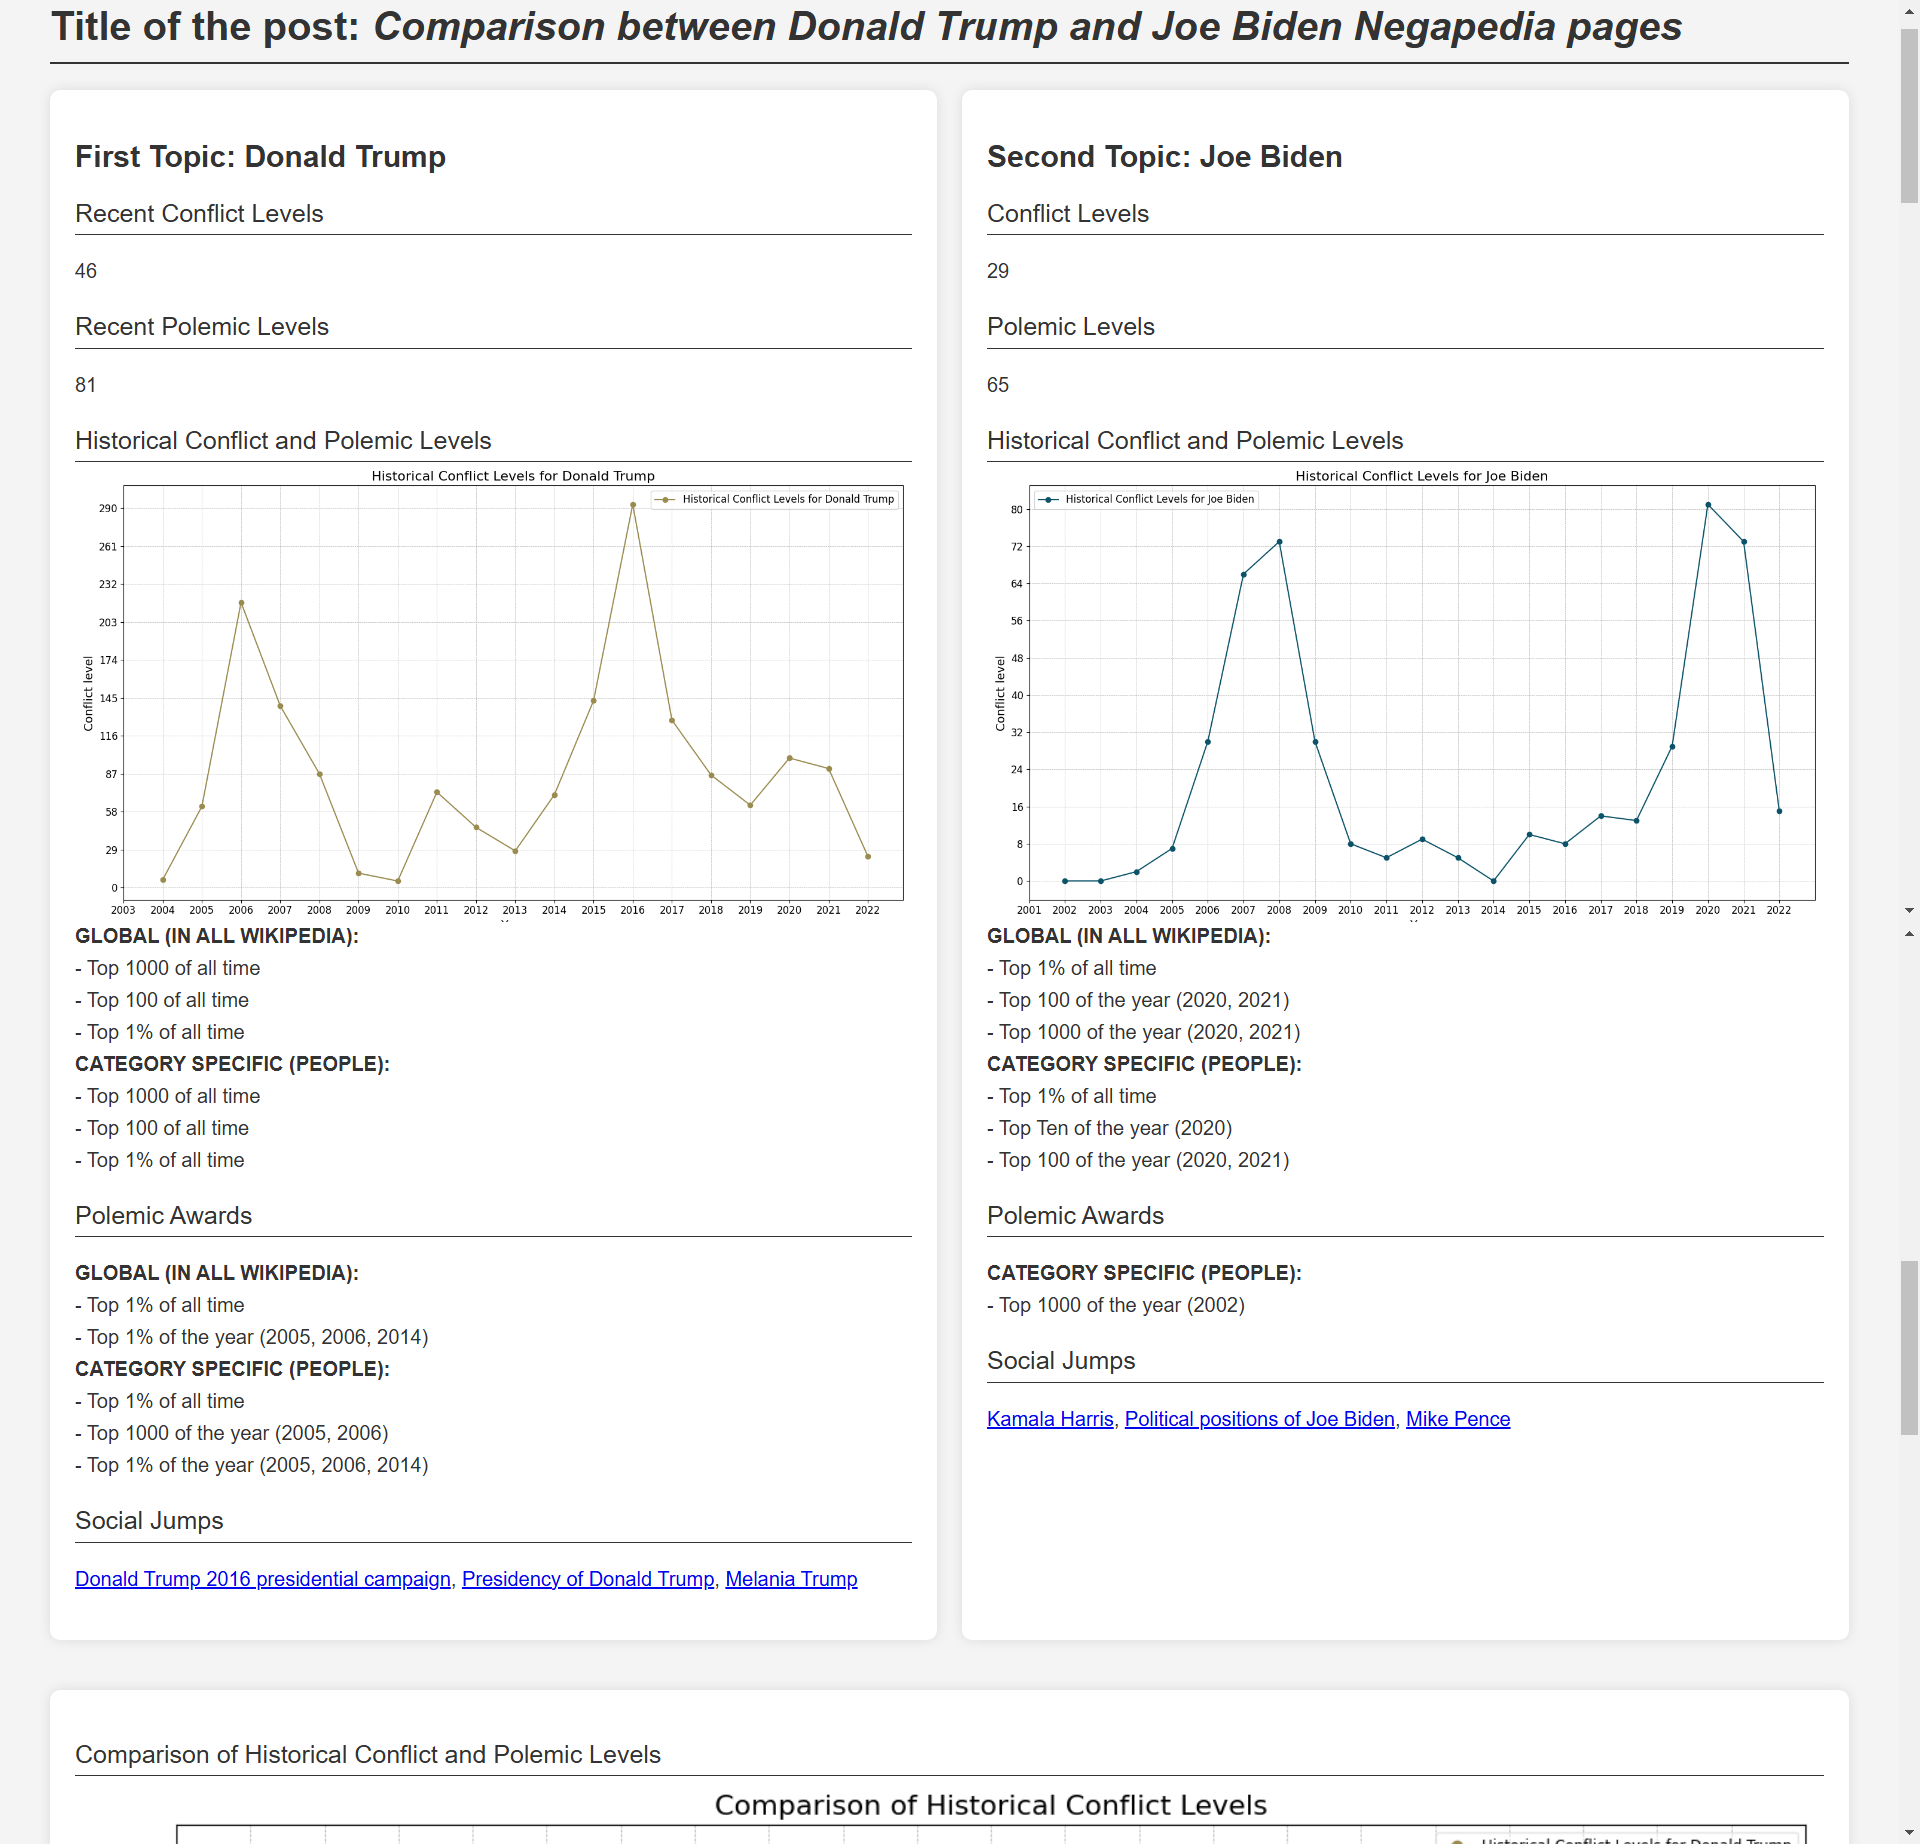
\includegraphics[width=0.8\textwidth, keepaspectratio]{images/web_page_negapedia_comparison_post_screenshot.png}
        \end{center}
    \end{frame}
    
    \begin{frame}{Facebook Post}
        Post generated using \textbf{Negapedia Module} in \textbf{Ranking Mode}.
        \vspace{-0.12cm}
        \begin{center}
            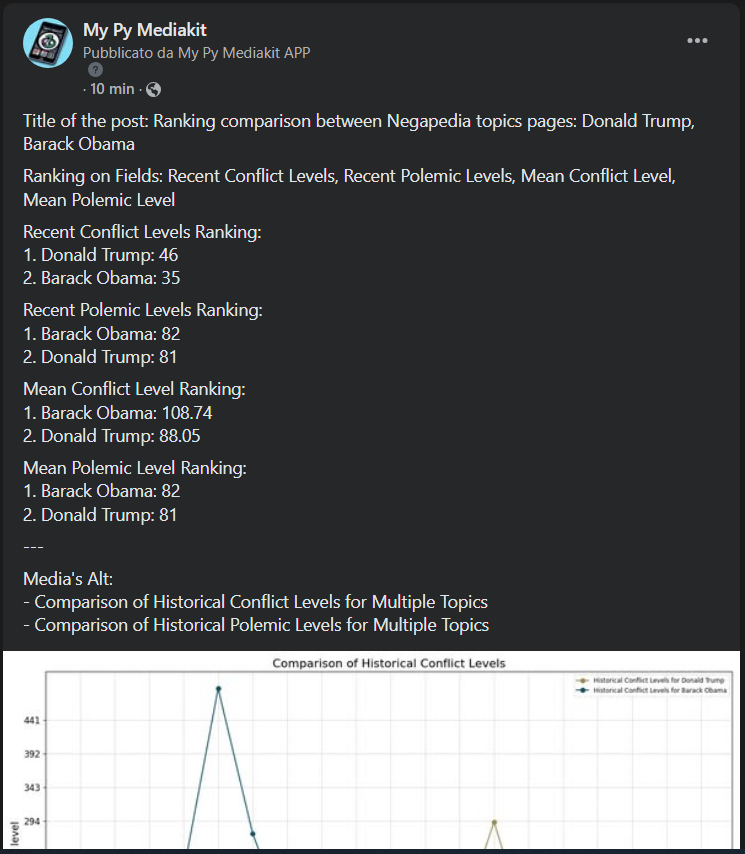
\includegraphics[width=0.8\textwidth, keepaspectratio]{images/facebook_negapedia_ranking_post_screenshot.png}
        \end{center}
    \end{frame}


\section{Contributions and Future Work}
    \begin{frame}{Contributions}
        \begin{block}{Key Contributions of SMKIT}
            \begin{itemize}
                \item \textbf{Modular Framework:}
                    \begin{itemize}
                        \item Provides a Generic Module for handling Open Graph metadata.
                        \item Includes a specialized Negapedia module tailored to process unique data metrics.
                    \end{itemize}
                \item \textbf{Cross-Platform Automation:}
                    \begin{itemize}
                        \item Supports automated posting to multiple platforms, including Facebook and Twitter.
                    \end{itemize}
                \item \textbf{Open-Source Tool:}
                    \begin{itemize}
                        \item Designed as an extensible framework to encourage community contributions and integration with additional platforms.
                    \end{itemize}
            \end{itemize}
        \end{block}
    \end{frame}

    \begin{frame}{Future Work}
        \begin{exampleblock}{Potential Extensions}
            \begin{itemize}
                \item \textbf{Additional Modules:}
                    \begin{itemize}
                        \item Develop specialized modules for other interesting platforms.
                    \end{itemize}
                \item \textbf{Additional Channels:}
                    \begin{itemize}
                        \item Develop specialized connectors for other channels, such as Instagram or LinkedIn.
                    \end{itemize}
                \item \textbf{Enhanced Analytics:}
                    \begin{itemize}
                        \item Integrate advanced analytics to track post performance.
                    \end{itemize}
                \item \textbf{Improved User Interface:}
                    \begin{itemize}
                        \item Design and implement a graphical user interface (GUI) to make SMKIT more accessible and user-friendly.
                    \end{itemize}
            \end{itemize}
        \end{exampleblock}
    \end{frame}


\section{Conclusion}
    \begin{frame}{Conclusion}
        \begin{itemize}
            \item \textbf{The Problem:}
                Managing and posting web content manually is inefficient and inconsistent.
            \item \textbf{The Solution:}
                SMKIT provides a modular, automated tool for extracting metadata and publishing across multiple platforms.
            \item \textbf{Key Results:} Successfully demonstrated automation capabilities.
        \end{itemize}

        \begin{block}{Closing Statement}
            SMKIT is a significant step towards automating social media and web content management, with potential for further innovation and adaptability.
        \end{block}
    \end{frame}


\begin{emptyframe}
     \textbf{ \textit{Thank you!} }
\end{emptyframe}

\appendix
    
\end{document}